\documentclass{article}
\usepackage{graphicx}
\usepackage{float}
\usepackage[export]{adjustbox}
\usepackage{tabularx}
\usepackage{multirow}
\usepackage{multicol}
\usepackage{booktabs}
\usepackage[table]{xcolor}
\usepackage{natbib}
\setcitestyle{round}

\title{Assignment 2, Replication and extension of Muchlinski et al. (2016)\\Random forest vs logistic regression}
\date{October 15, 2020}
\author{Eve Fleisig, Jordan Klein, Matthew Sun}

\begin{document}

\maketitle

\section*{Part 1: Replication}

We begin by replicating the separation plots from \cite{muchlinski2016comparing}
using their updated replication materials (Fig.~\ref{fig:separation}). Our separation plots for the logistic regression models by Fearon and Laitin (2003), Collier and Hoeffler (2004), and Hegre and Sambanis (2006) are identical to those from Muchlinski et al.'s original paper, but notably, our separation plot for random forests identifies 2 false positives while that from Muchlinski et al's original paper does not identify any. These results align with those produced by Mulchinski et al. in their own replication \citep{muchlinski_2019}. Our findings refute Muchlinski et al's initial assertion that random forests is uniquely impervious to Type II compared to logistic regression.

We continue by replicating the ROC curves from \cite{muchlinski2016comparing} (Fig.~\ref{fig:ROC}). Like \cite{muchlinski2016comparing}, we find random forests has an AUC of .91, but as explained by \cite{wang_comparing_2019}, the ROC curve in Muchlinksi et al's original paper implies an AUC of .97. Our redrawing of the ROC curve to be consistent with an AUC of .91 aligns with Muchlinski et al's replication \citep{muchlinski_2019}. In contrast, our ROC curves for logistic regression and L1-penalized logistic regression do not change very much compared to \cite{muchlinski2016comparing}. However, we note that Muchlinski et al. do not provide updated calculations of AUC in their replication \citep{muchlinski_2019}. We therefore recalculate AUC for all models and find those for uncorrected and penalized logistic regression to be slightly higher than those shown in Muchlinski et al's original paper. These results demonstrate that the gap in performance between random forests and logistic regression is substantially smaller than they report.

As suggested by \cite{neunhoeffer_how_2019}, the out-of-sample analysis reported by \cite{muchlinski2016comparing} does not match that from the article's original replication materials \citep{muchlinski_replication_2015}. In replicating the analysis from Muchlinski et al's updated materials \citep{muchlinski_2019}, using a threshold for positive prediction of .5 we find that the logistic regression models all fail to predict any civil war (Table~\ref{tab:oos}), as they originally reported. However, random forests performs slightly better, correctly predicting 10 rather than 9 out of 20 civil wars. Such a small difference however is not of import, especially because of the randomness inherent in both the imputation and random forests procedures used \citep{muchlinski_seeing_2019}. 

\begin{figure}[H]
     \makebox[\textwidth][c]{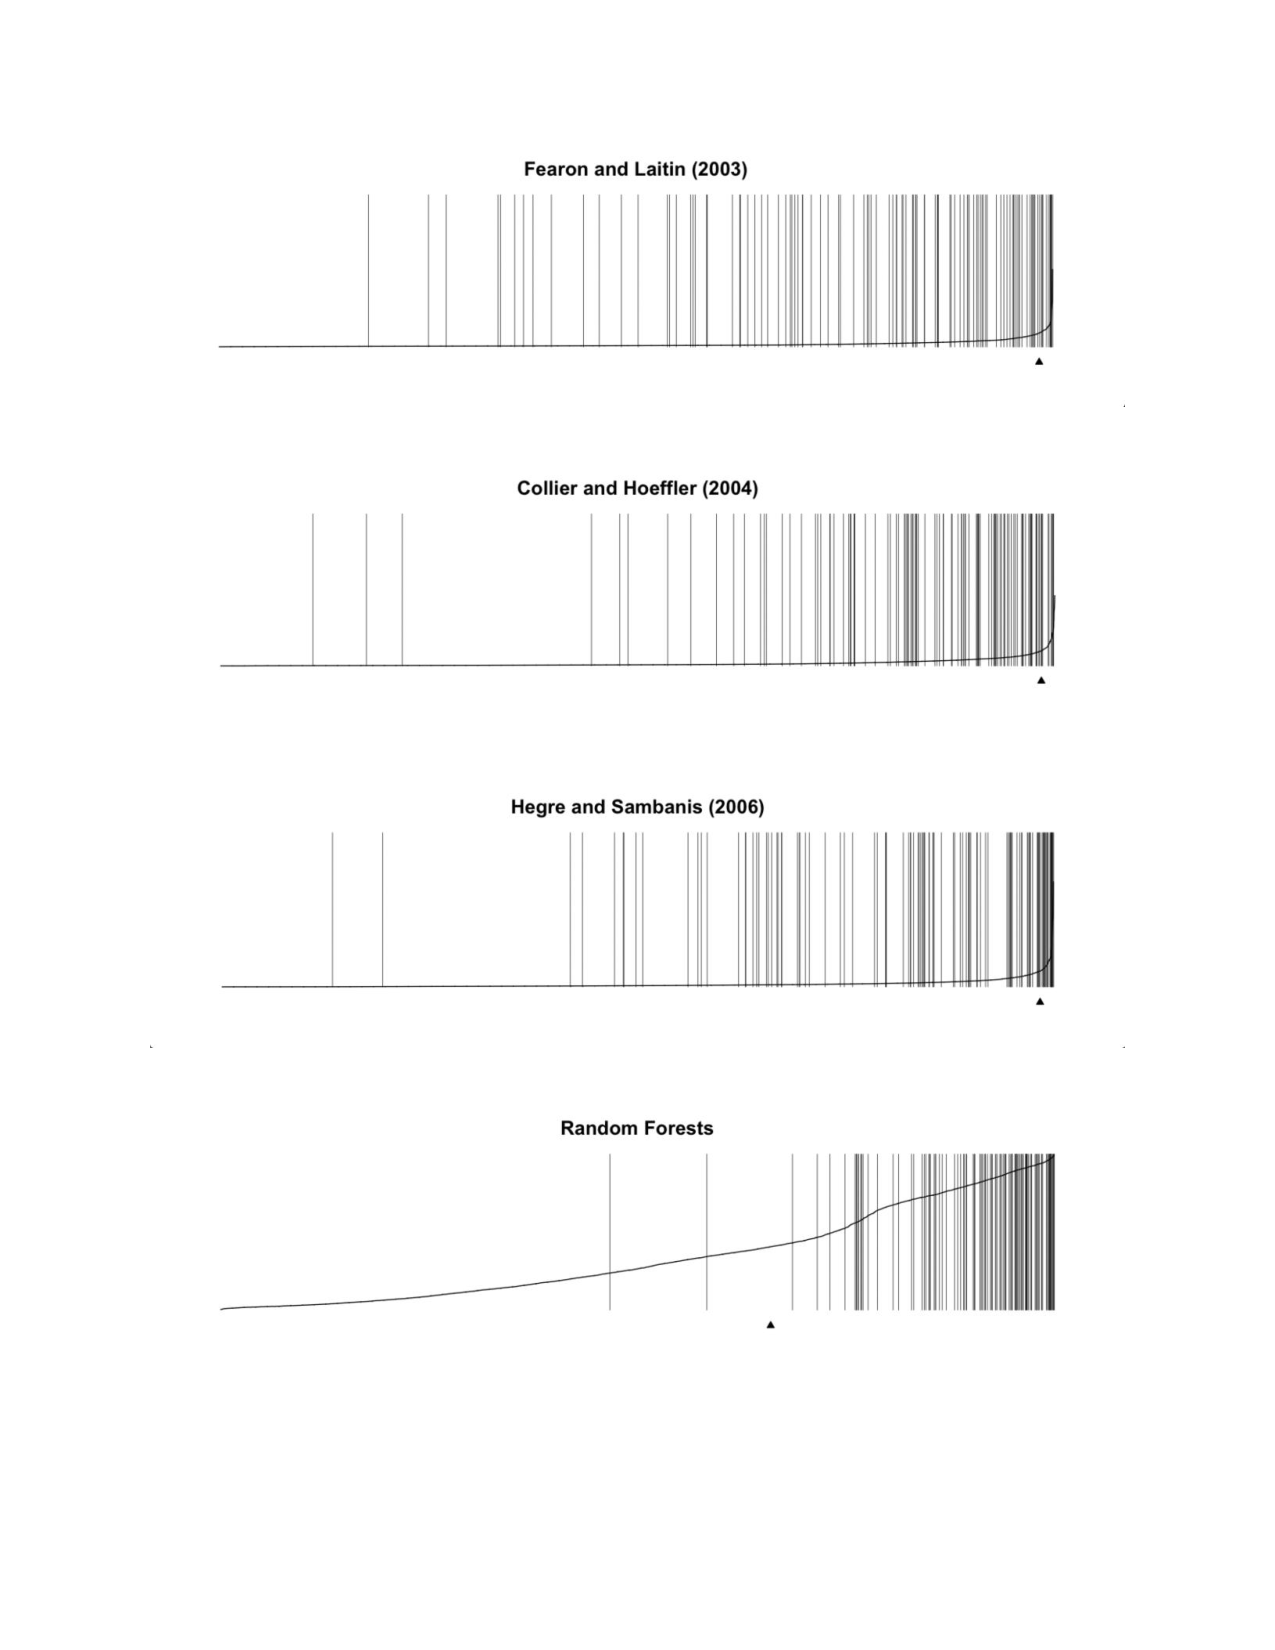
\includegraphics[width=1.3\textwidth]{Figures/figure1.pdf}}%
    \caption{Separation plot for all classifiers.}
\label{fig:separation}
\end{figure}

\begin{figure}[H]
    \makebox[\textwidth][c]{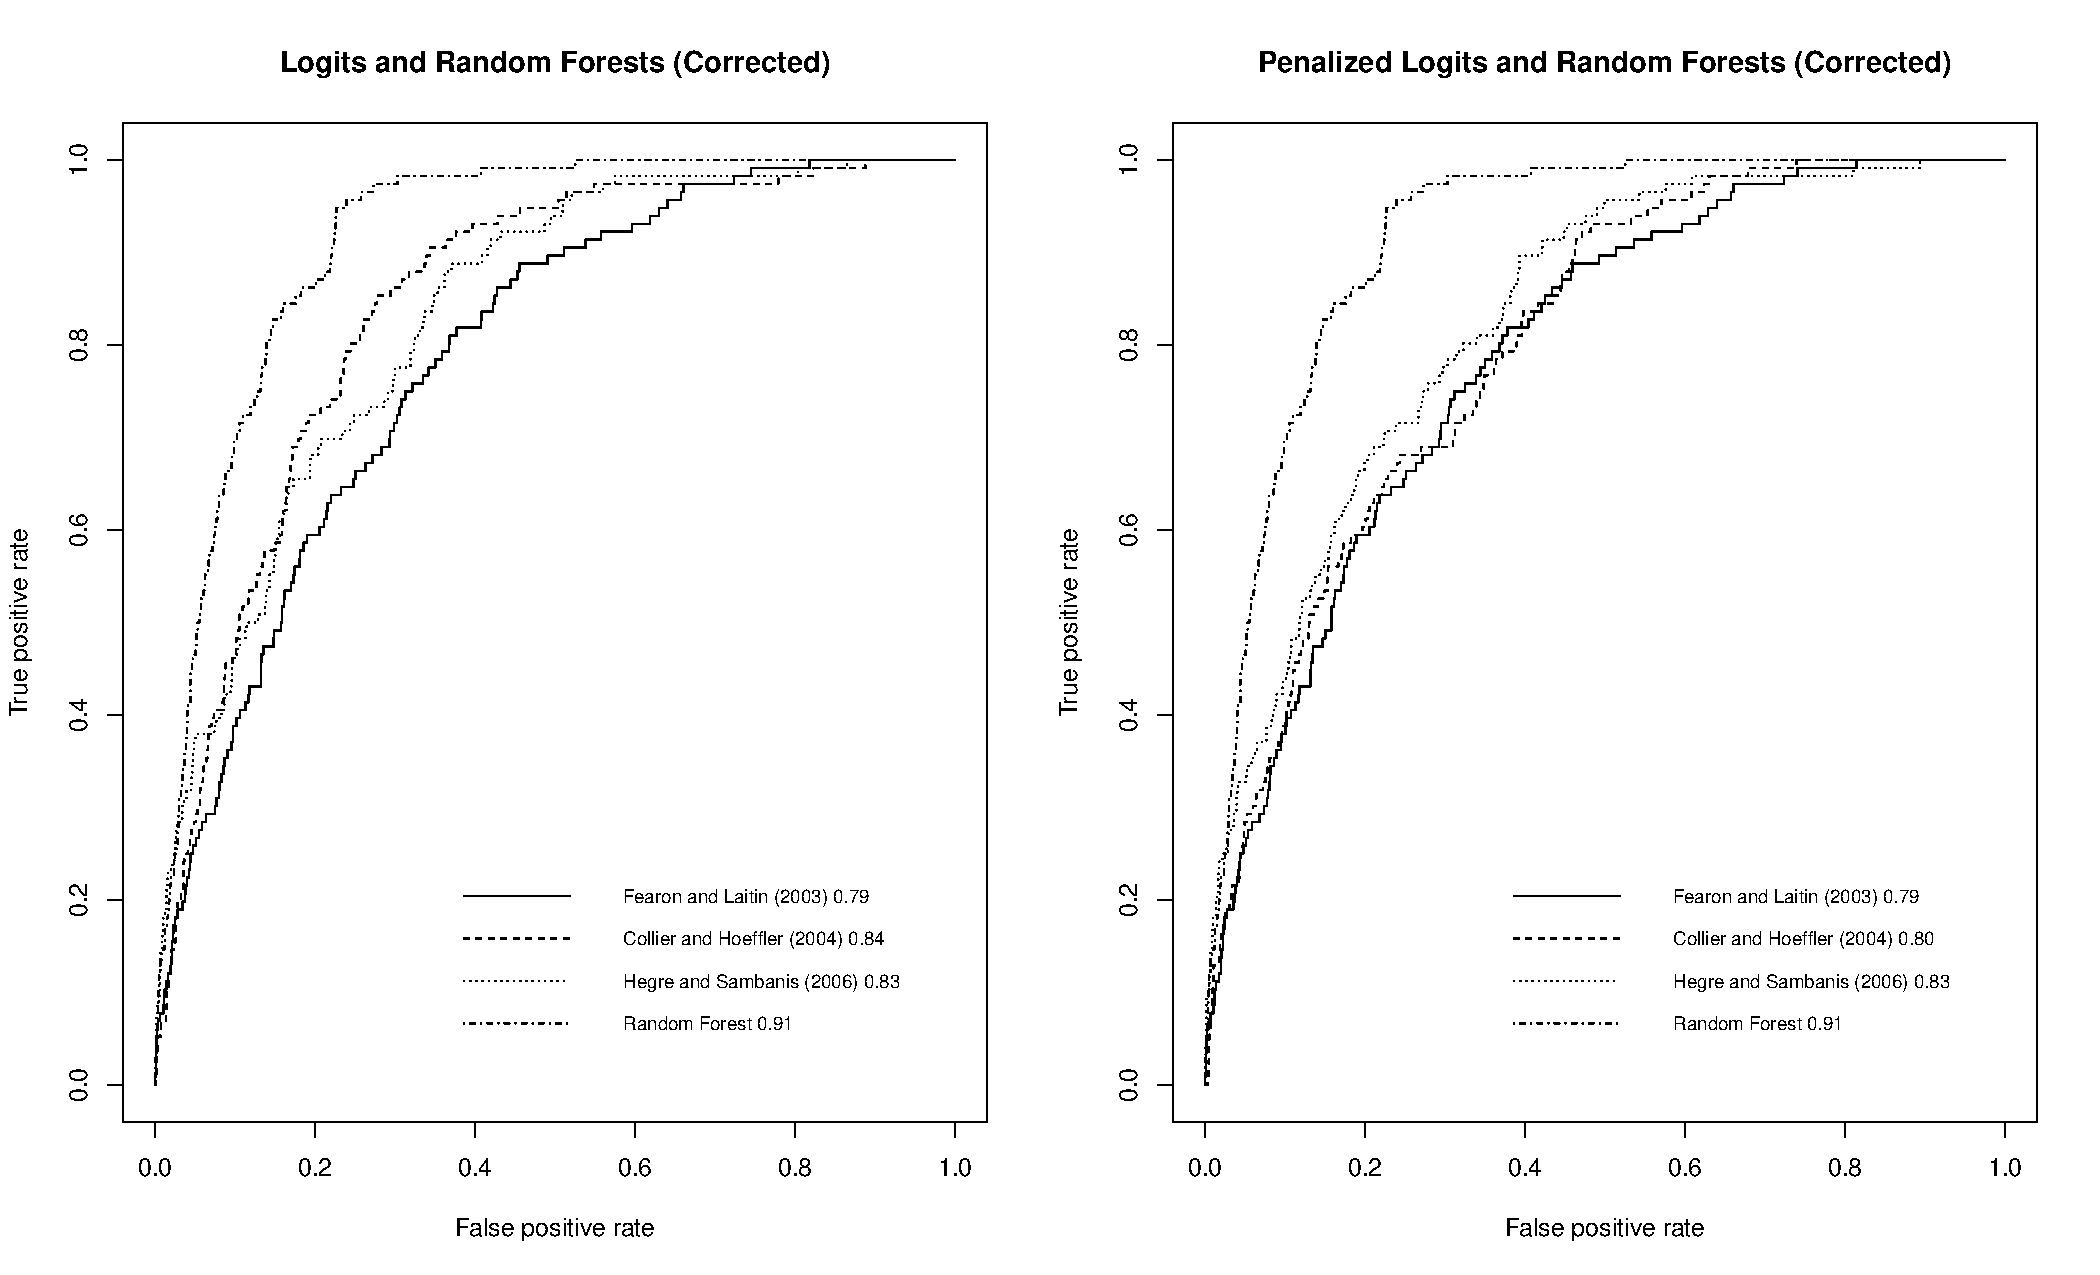
\includegraphics[width=1.4\textwidth]{Figures/figure2.pdf}}%
    \caption{ROC curves for all classifiers.}
\label{fig:ROC}
\end{figure}

\begin{table}[H]
\centering
\caption{Predicted probability of civil war onset: Logistic Regression and Random Forests}
\resizebox{\linewidth}{!}{
    \begin{tabular}{lccccc}
    \toprule
    \multicolumn{6}{c}{Models and predicted probability of civil war onset} \\
    \cmidrule(l{3pt}r{3pt}){1-6}
Country & Year & Fearon and Latin (2003) & Collier and Hoeffler (2004) & Hegre and Sambanis (2006) & Random Forest\\
    \midrule
    \rowcolor{gray!6}  Afghanistan & 2001 & 0.01 & 0.00 & 0.00 & 0.06\\
Angola & 2001 & 0.01 & 0.01 & 0.02 & 0.71\\
    \rowcolor{gray!6}  Burundi & 2001 & 0.03 & 0.00 & 0.02 & 0.09\\
Guinea & 2001 & 0.01 & 0.00 & 0.01 & 0.07\\
    \rowcolor{gray!6}  Rwanda & 2001 & 0.01 & 0.00 & 0.01 & 0.05\\
\addlinespace
Uganda & 2002 & 0.02 & 0.02 & 0.02 & 0.93\\
    \rowcolor{gray!6}  Liberia & 2003 & 0.02 & 0.04 & 0.03 & 0.98\\
Iraq & 2004 & 0.03 & 0.01 & 0.03 & 0.16\\
    \rowcolor{gray!6}  Uganda & 2004 & 0.01 & 0.00 & 0.01 & 0.45\\
Afghanistan & 2005 & 0.03 & 0.00 & 0.02 & 0.14\\
    \addlinespace
    \rowcolor{gray!6}  Chad & 2006 & 0.02 & 0.04 & 0.03 & 0.98\\
Somalia & 2007 & 0.06 & 0.04 & 0.10 & 0.96\\
    \rowcolor{gray!6}  Rwanda & 2009 & 0.02 & 0.04 & 0.03 & 0.99\\
Libya & 2011 & 0.02 & 0.04 & 0.02 & 0.95\\
    \rowcolor{gray!6}  Syria & 2012 & 0.01 & 0.00 & 0.00 & \vphantom{1} 0.06\\
    \addlinespace
Syria & 2012 & 0.01 & 0.00 & 0.00 & 0.06\\
    \rowcolor{gray!6}  Democratic Republic of the Congo & 2013 & 0.01 & 0.00 & 0.00 & 0.04\\
Iraq & 2013 & 0.02 & 0.04 & 0.02 & 0.96\\
    \rowcolor{gray!6}  Nigeria & 2013 & 0.02 & 0.04 & 0.03 & 0.96\\
Somalia & 2014 & 0.05 & 0.04 & 0.11 & 0.99\\
    \bottomrule
\end{tabular}}
\label{tab:oos}
\end{table}

\begin{figure}[H]
    \makebox[\textwidth][c]{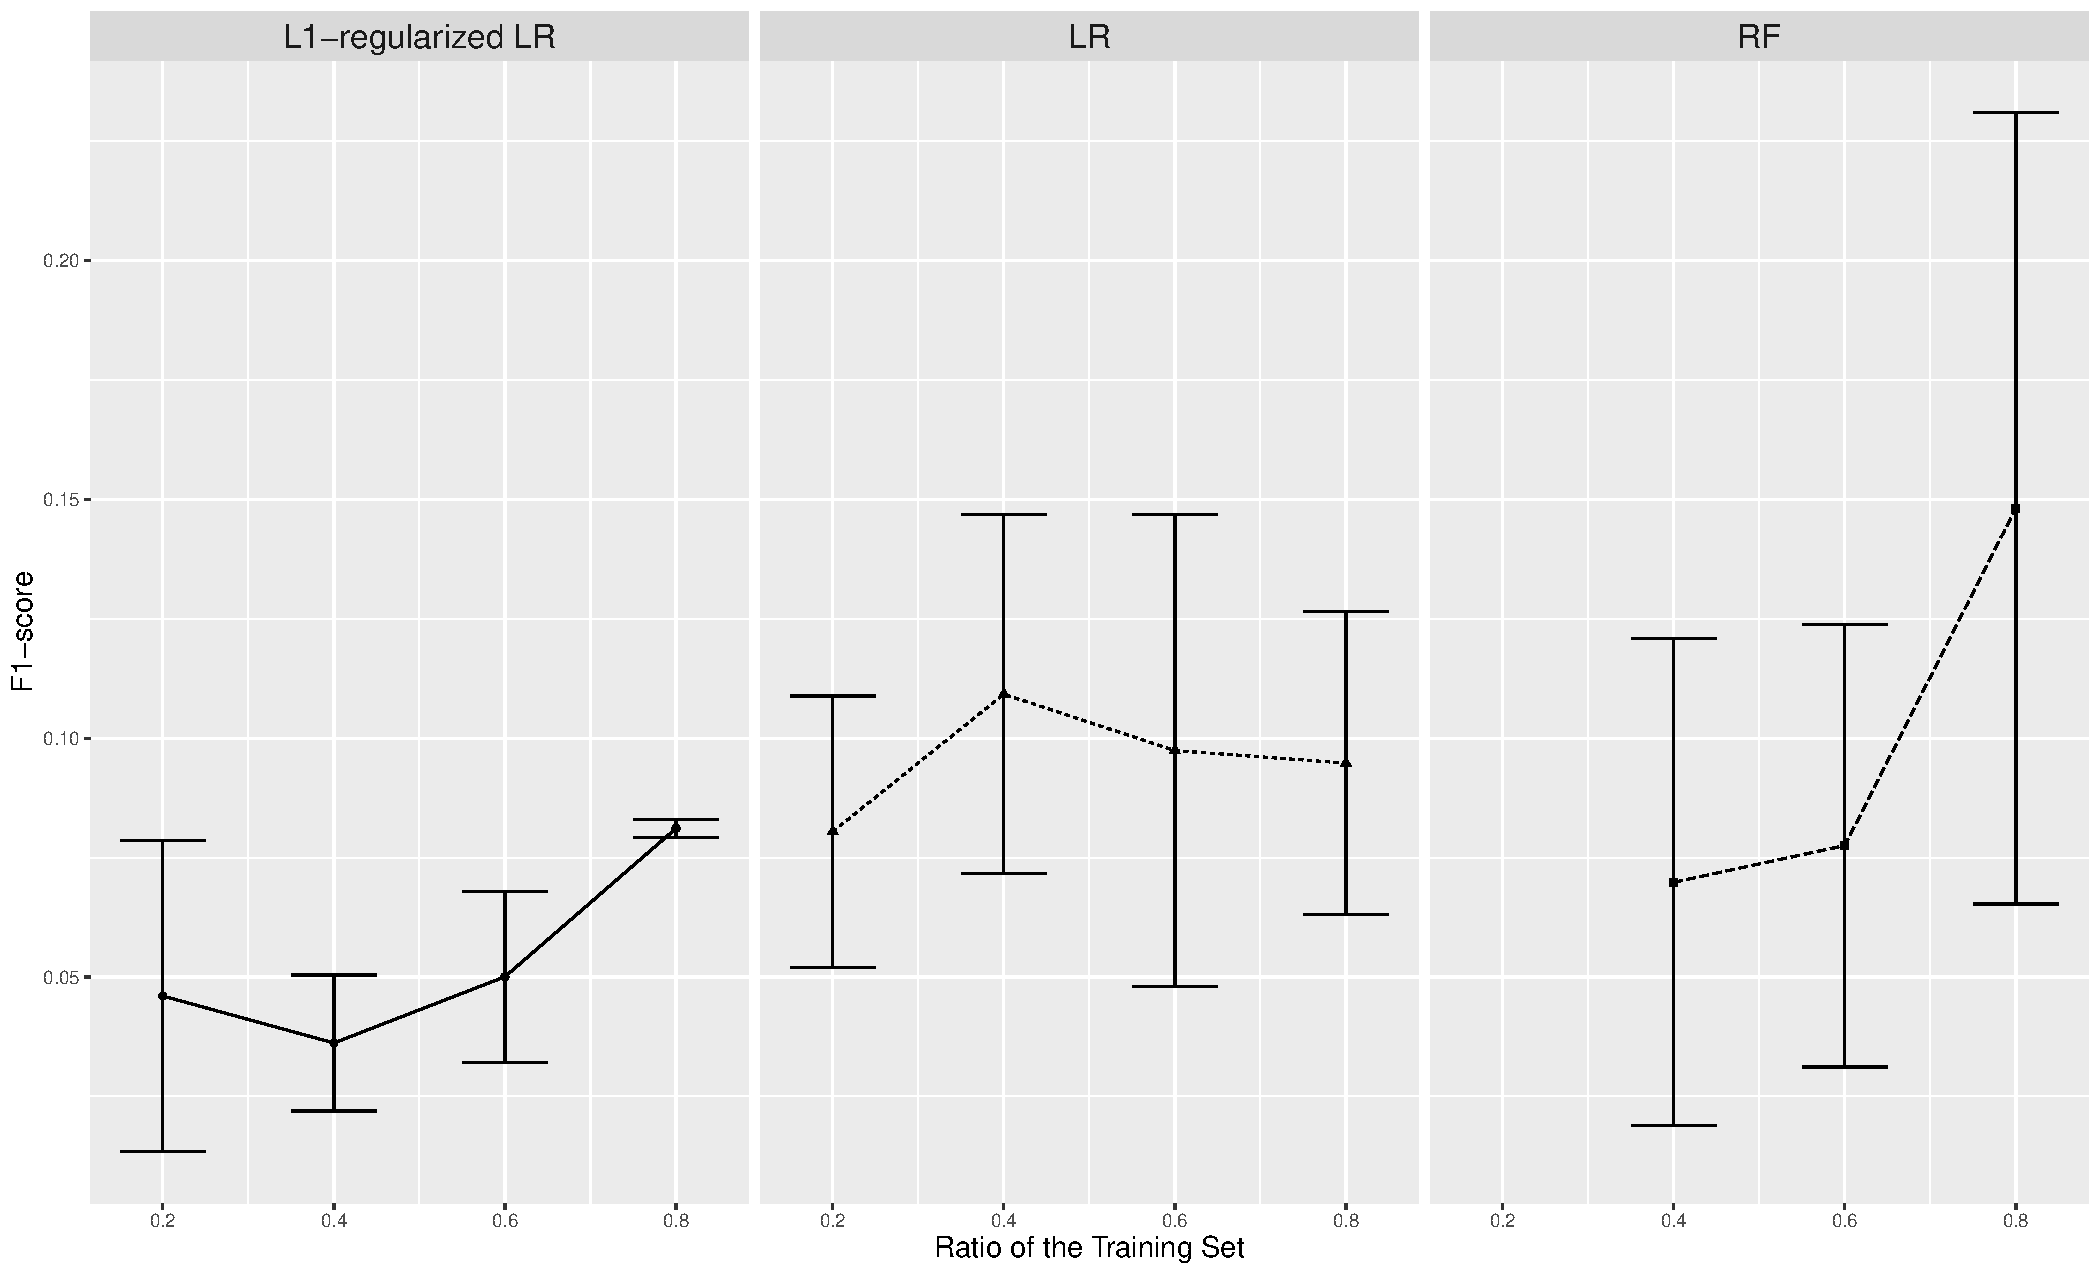
\includegraphics[width=1.4\textwidth]{Figures/figure3.pdf}}%
    \caption{ROC curves for all classifiers.}
\label{fig:f1}
\end{figure}

\newpage

\section*{Part 2: Extension}
\subsection*{Introduction}
A central issue in the methodology proposed by Muchlinski et al. to evaluate civil war onset prediction is the assumption that the onset of a civil war is a binary variable, such that civil war either occurred or did not occur in a given year. However, real-life civil war onset is rarely so discrete: skirmishes and widespread civil unrest often precede the onset of declared war, and intrastate conflicts may not qualify as civil war depending on the subjective criteria used. We questioned whether the results that Muchlinski et al. obtained might be dependent on the arbitrary cutoff for civil war on which their predictions depend.

A related question is whether Muchlinski et al.'s results hold with the use of lag models, predicting the number of deaths per capita given the number of deaths per capita in the previous year. In addition, lagged datasets correspond more closely to real-world applications in which data about the history of a given country is already available.

To investigate these possibilities, we examined whether continuous prediction of the degree of state violence given data from the previous year would affect the relative predictive power of random forests and regression models. Measuring the degree of unrest by the number of deaths per capita in a given year, we trained a random forest and a linear regression model\footnote{Because this task predicts a continuous outcome (deaths per capita), we use a linear regression model rather than the logistic regression model used by Muchlinski et al.} to examine their ability to predict the degree of violence.

We also examined whether methods improving on traditional random forests improve classifier results. Discrepancies between the performance of different tree-based models could suggest that arguments about the relative merits of families of classifiers are highly dependent on the specific models used. We compared the performance of the random forest and logistic regression models to LightGBM, a faster variant of gradient boosting decision trees \citep{ke2017lightgbm}.



\subsection*{Methods}
The Uppsala Conflict Data Program (UCDP) measures the number of deaths per country due to several types of conflict. We used the number of deaths per country due to intrastate violence, which the UCDP defines as violence between a government and rebel troops without the involvement of foreign governments with troops, and internationalized intrastate violence, which the UCDP defines as violence between a government and rebel troops with some involvement of foreign governments with troops.

We excluded deaths due to extrasystemic violence (between a state and a non-state outside its territory) and interstate violence as inapplicable to civil war. We then used the United Nations' population data to determine the number of deaths due to intrastate violence per capita for each country in each year from 1989 to 2000.

For each year from 1992 to 2000, the validation set was the prediction for that year and the training set consisted of the data from all previous years. All models used the same training features that Muchlinski et al. used and the number of deaths per capita in the previous year. We found that predictions using the previous two or three years performed worse than the previous year alone. As a baseline, we used a model that simply predicted the same number of deaths as the previous year in all cases.

Our code is available at \texttt{github.com/jordan-klein/muchlinksi\_replication}.

\subsection*{Results}
After training the random forest, linear regression, and LightGBM models, we found the root mean squared logarithmic error (RMSLE) of each model's casualty predictions (Table \ref{table:results}). The LightGBM model had the lowest error rate (0.00072), followed by the linear regression model (0.00074) and then the random forest (0.000087).

\begin{table}[H]
\centering
\caption{Root mean squared log error of casualty prediction.}
\resizebox{\linewidth}{!}{
    \begin{tabular}{lcccc}
    \toprule
    \multicolumn{5}{c}{RMSLE of casualty prediction} \\
    \cmidrule(l{3pt}r{3pt}){1-5}
Year & Baseline & Random Forest & LightGBM & Linear Regression\\
    \midrule
    \rowcolor{gray!6}  1992 &	0.00009& 0.000044 &	0.000035 &	0.000048\\
    1993 & 0.00007&	0.000083 &	0.000062 &	0.000072\\
    \rowcolor{gray!6}  1994 & 0.00008&	0.000076 &	0.000058 &	0.000045\\
    1995 & 0.00005&	0.000051 &	0.000049 &	0.000036\\
    \rowcolor{gray!6}  1996 &0.00005&	0.000045 &	0.000041 &	0.000039\\
    1997 &0.00027&	0.000273 &	0.000272 &	0.000273\\
    \rowcolor{gray!6}  1998 &0.00019&	0.000114 &	0.000070 &	0.000077\\
    1999 &0.00008&	0.000063 &	0.000041 &	0.000049\\
    \rowcolor{gray!6}  2000 &0.00003 &	0.000032 &	0.000022 &	0.000025\\
    \addlinespace
    Mean & 0.00010 & 0.000087 & 0.000072 & 0.000074\\
    \bottomrule
\end{tabular}}
\label{table:results}
\end{table}

\begin{figure}[H]
     \makebox[\textwidth][c]{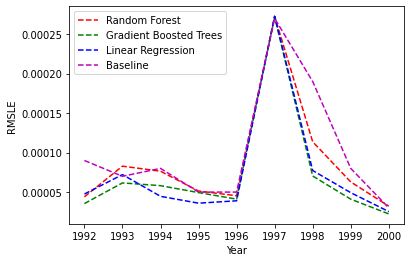
\includegraphics[width=0.9\textwidth]{Figures/replication_results.png}}%
    \caption{RMSLE of casualty predictions.}
\label{fig:RMSLE}
\end{figure}

These results contrast with Muchlinski et al., who found that random forests outperformed several types of logistic regression. In fact, the random forest model had the highest or tied for the highest error in eight of the nine years examined. This discrepancy suggests that Muchlinski et al.'s results hinge on the structure of the problem: the binary variable they predict, the metrics used to evaluate binary classification, and the absence of lag models. When predicting a continuous variable from a lagged dataset, random forests no longer outperform regression models. In addition, the fact that gradient boosted trees outperformed the other models suggest that broad conclusions about tree-based methods are dependent on the exact model used in a given scenario.

Ultimately, the differences between Muchlinski et al.'s results and ours underscore the notion that sweeping conclusions about the relative merits of different classifiers rely heavily on the presentation of the problem, particularly the features used by the models and how predicted classes are defined.

\vspace{20px}

\nocite{ucdp}
\renewcommand\refname{Bibliography}

\bibliographystyle{plainnat} % or try abbrvnat or unsrtnat
\bibliography{refs}
\end{document}
